% Options for packages loaded elsewhere
\PassOptionsToPackage{unicode}{hyperref}
\PassOptionsToPackage{hyphens}{url}
\PassOptionsToPackage{dvipsnames,svgnames,x11names}{xcolor}
%
\documentclass[
  english,
  a4paper,
]{article}
\usepackage{amsmath,amssymb}
\usepackage{lmodern}
\usepackage{iftex}
\ifPDFTeX
  \usepackage[T1]{fontenc}
  \usepackage[utf8]{inputenc}
  \usepackage{textcomp} % provide euro and other symbols
\else % if luatex or xetex
  \usepackage{unicode-math}
  \defaultfontfeatures{Scale=MatchLowercase}
  \defaultfontfeatures[\rmfamily]{Ligatures=TeX,Scale=1}
\fi
% Use upquote if available, for straight quotes in verbatim environments
\IfFileExists{upquote.sty}{\usepackage{upquote}}{}
\IfFileExists{microtype.sty}{% use microtype if available
  \usepackage[]{microtype}
  \UseMicrotypeSet[protrusion]{basicmath} % disable protrusion for tt fonts
}{}
\makeatletter
\@ifundefined{KOMAClassName}{% if non-KOMA class
  \IfFileExists{parskip.sty}{%
    \usepackage{parskip}
  }{% else
    \setlength{\parindent}{0pt}
    \setlength{\parskip}{6pt plus 2pt minus 1pt}}
}{% if KOMA class
  \KOMAoptions{parskip=half}}
\makeatother
\usepackage{xcolor}
\IfFileExists{xurl.sty}{\usepackage{xurl}}{} % add URL line breaks if available
\IfFileExists{bookmark.sty}{\usepackage{bookmark}}{\usepackage{hyperref}}
\hypersetup{
  pdftitle={TODO title},
  pdflang={en},
  colorlinks=true,
  linkcolor={blue},
  filecolor={Maroon},
  citecolor={blue},
  urlcolor={blue},
  pdfcreator={LaTeX via pandoc}}
\urlstyle{same} % disable monospaced font for URLs
\usepackage[margin=25mm]{geometry}
\usepackage{longtable,booktabs,array}
\usepackage{calc} % for calculating minipage widths
% Correct order of tables after \paragraph or \subparagraph
\usepackage{etoolbox}
\makeatletter
\patchcmd\longtable{\par}{\if@noskipsec\mbox{}\fi\par}{}{}
\makeatother
% Allow footnotes in longtable head/foot
\usepackage{footnote} % For some unknown reason, footnotehyper clashes with French
\makesavenoteenv{longtable}
\usepackage{graphicx}
\makeatletter
\def\maxwidth{\ifdim\Gin@nat@width>\linewidth\linewidth\else\Gin@nat@width\fi}
\def\maxheight{\ifdim\Gin@nat@height>\textheight\textheight\else\Gin@nat@height\fi}
\makeatother
% Scale images if necessary, so that they will not overflow the page
% margins by default, and it is still possible to overwrite the defaults
% using explicit options in \includegraphics[width, height, ...]{}
\setkeys{Gin}{width=\maxwidth,height=\maxheight,keepaspectratio}
% Set default figure placement to htbp
\makeatletter
\def\fps@figure{htbp}
\makeatother
\setlength{\emergencystretch}{3em} % prevent overfull lines
\providecommand{\tightlist}{%
  \setlength{\itemsep}{0pt}\setlength{\parskip}{0pt}}
\setcounter{secnumdepth}{5}
\newlength{\cslhangindent}
\setlength{\cslhangindent}{1.5em}
\newlength{\csllabelwidth}
\setlength{\csllabelwidth}{3em}
\newlength{\cslentryspacingunit} % times entry-spacing
\setlength{\cslentryspacingunit}{\parskip}
\newenvironment{CSLReferences}[2] % #1 hanging-ident, #2 entry spacing
 {% dont indent paragraphs
  \setlength{\parindent}{0pt}
  % turn on hanging indent if param 1 is 1
  \ifodd #1
  \let\oldpar\par
  \def\par{\hangindent=\cslhangindent\oldpar}
  \fi
  % set entry spacing
  \setlength{\parskip}{#2\cslentryspacingunit}
 }%
 {}
\usepackage{calc}
\newcommand{\CSLBlock}[1]{#1\hfill\break}
\newcommand{\CSLLeftMargin}[1]{\parbox[t]{\csllabelwidth}{#1}}
\newcommand{\CSLRightInline}[1]{\parbox[t]{\linewidth - \csllabelwidth}{#1}\break}
\newcommand{\CSLIndent}[1]{\hspace{\cslhangindent}#1}

%%%%%%%% START HEADER PARTIAL %%%%%%%%%%%%

% Formatting of tables & knitr::kable and kableExtra functionality
\usepackage{float}
\usepackage{colortbl}
\usepackage{pdflscape}
\usepackage{tabu}
\usepackage{threeparttable}

% Line numbering

% endfloat stuff

% fancyhdr pagestyle

% Environment for keywords
\makeatletter
\newcommand\keywordsname{Keywords}
\newenvironment*{keywords}[1][\keywordsname]{\if@twocolumn \else \small \quotation \fi \begin{center} \textbf{\textit{#1} \\}}{\end{center}\if@twocolumn \else \small \endquotation \fi}
\newenvironment*{keywordsinline}[1][\keywordsname]{\if@twocolumn \else \small \quotation \fi \begin{center} \textbf{\textit{#1}: }}{\end{center}\if@twocolumn \else \small \endquotation \fi}
\makeatother

% Environment for abstract that takes new abstract name
\newenvironment{renameableabstract}[1][\abstractname]{\let\oldabstractname\abstractname \renewcommand{\abstractname}{#1} \begin{abstract}}{\end{abstract} \renewcommand{\abstractname}{\oldabstractname}}

%%%%%%%% END HEADER PARTIAL %%%%%%%%%%%%

\usepackage{booktabs}
\usepackage{longtable}
\usepackage{array}
\usepackage{multirow}
\usepackage{wrapfig}
\usepackage{float}
\usepackage{colortbl}
\usepackage{pdflscape}
\usepackage{tabu}
\usepackage{threeparttable}
\usepackage{threeparttablex}
\usepackage[normalem]{ulem}
\usepackage{makecell}
\usepackage{xcolor}
\ifXeTeX
  % Load polyglossia as late as possible: uses bidi with RTL langages (e.g. Hebrew, Arabic)
  \usepackage{polyglossia}
  \setmainlanguage[]{}
\else
  \usepackage[english,main=english]{babel}
% get rid of language-specific shorthands (see #6817):
\let\LanguageShortHands\languageshorthands
\def\languageshorthands#1{}
\fi
\ifLuaTeX
  \usepackage{selnolig}  % disable illegal ligatures
\fi

\title{TODO title}

%%%%%%% START AUTHOR PARTIAL %%%%%%%%%%%%%%%

%%%%% Authors, affiliations and author notes stuff %%%%%

% Macros for creating and referencing stored reference
\makeatletter
\def\MyNewLabel#1#2#3{\expandafter\gdef\csname #1@#2\endcsname{#3}}

\def\MyRef#1#2{\@ifundefined{#1@#2}{???}{\csname #1@#2\endcsname}}

\newcommand*\ifcounter[1]{%
  \ifcsname c@#1\endcsname
    \expandafter\@firstoftwo
  \else
    \expandafter\@secondoftwo
  \fi
}
\makeatother

% Create labels for Addresses if the are given by code
\MyNewLabel{ADDRTXT}{Stanford}{Stanford University}

% Create labels for Footnotes if they are given by code
\MyNewLabel{ANOTETXT}{corresp}{Corresponding author. Email: \href{mailto:vboyce@stanford.edu}{\nolinkurl{vboyce@stanford.edu}}}

%%% Special footnotes for addresses and author footnotes
\usepackage{bigfoot}
\DeclareNewFootnote{Addr}[arabic] % Only used for NOT authblk
\DeclareNewFootnote{ANote}[fnsymbol]

%%% Address and author notes as a function of format %%%
 % Use authblk for affiliations %%%%%%%%%%%
\usepackage{authblk}

% Always separate by commas
\renewcommand\Authsep{, }
\renewcommand\Authand{, }
\renewcommand\Authands{, }

% Counter for addresses and footnotes
\newcounter{addrcnt}

% thanks definition that doesnt produce superscript marks
\makeatletter
\newcommand*\createaddrlblbycode[1]{%
  \ifcounter{ADDRLBL@#1}
    {}
    {\refstepcounter{addrcnt}\newcounter{ADDRLBL@#1}\setcounter{ADDRLBL@#1}{\value{addrcnt}}}%
}

\newcommand*\addrlblbycode[1]{\arabic{ADDRLBL@#1}}

\newcommand*\addrbycode[1]{%
  \ifcounter{ADDR@#1}
    {}
    {\newcounter{ADDR@#1}%
     \affil[\addrlblbycode{#1}]{\MyRef{ADDRTXT}{#1}}}%
}

\newcommand*\createanotelblbycode[1]{%
  \ifcounter{ANOTELBL@#1}
    {}
    {\refstepcounter{footnoteANote}\newcounter{ANOTELBL@#1}\setcounter{ANOTELBL@#1}{\value{footnoteANote}}}%
}

\newcommand*\anotelblbycode[1]{\fnsymbol{ANOTELBL@#1}}

\newcommand*\anotebycode[1]{%
  \ifcounter{ANOTE@#1}
    {}
    {\newcounter{ANOTE@#1}%
     \footnotetextANote[\value{ANOTELBL@#1}]{\MyRef{ANOTETXT}{#1}}}%
}
\makeatother


\createaddrlblbycode{Stanford}


\createanotelblbycode{corresp}

\author[%
\addrlblbycode{Stanford}%
,%
$\anotelblbycode{corresp}$%
]{Veronica Boyce}

\addrbycode{Stanford}


\createaddrlblbycode{Stanford}



\author[%
\addrlblbycode{Stanford}%
]{Robert Hawkins}

\addrbycode{Stanford}


\createaddrlblbycode{Stanford}



\author[%
\addrlblbycode{Stanford}%
]{Noah D. Goodman}

\addrbycode{Stanford}


\createaddrlblbycode{Stanford}



\author[%
\addrlblbycode{Stanford}%
]{Michael C. Frank}

\addrbycode{Stanford}


%endif(authblk)

%%%%%%%%% END AUTHOR PARTIAL %%%%%%%%

\date{}

\begin{document}
\maketitle

%%%%%%%%%% START AFTER TITLE PARTIAL %%%%%%%%%%%%%
\anotebycode{corresp}


%%%%%%%%%% END AFTER TITLE PARTIAL %%%%%%%%%%%%%


\begin{otherlanguage}{english}

\begin{abstract}
\emph{This is an abstract in italics.}

This is the second paragraph not in italics.

\end{abstract}

\end{otherlanguage}

\begin{otherlanguage}{english}

\begin{keywords}
One keyword; Yet another keyword

\end{keywords}

\end{otherlanguage}

\hypertarget{introduction}{%
\section{Introduction}\label{introduction}}

\begin{itemize}
\item
  communication is important and takes place in non-dyadic situations
\item
  one interesting thing about comm is ad-hoc expressions, adaptation to speaker/ listener pairs
\item
  prior work has focused a lot on dyads: what happens with more people? Do theories predict anything?
\item
  groups also vary in compositional type aspects so mimics of these might matter
\item
  do we want to set up other theoretical frames? do I need to read more about theory??
\end{itemize}

Verbal communication is an integral part of our daily lives. We coordinate schedules with partners, socialize with friends over board games, learn and teach in seminar classes, and listen to podcasts. Communicative environments range in size from one-on-one dialogue to broadcast communication to large groups, but the goal of efficient communication is shared across these (\protect\hyperlink{ref-traum2004}{Traum 2004}, \protect\hyperlink{ref-branigan2006}{\textbf{branigan2006?}}, \protect\hyperlink{ref-ginzburg2005}{\textbf{ginzburg2005?}}). Shared referring expressions are a necessity for efficient communication; a thing or an idea needs some sort of name that the interlocutors will jointly understand. In many cases, there are widely shared conventionalized expressions for objects or ideas, but in other cases, spontaneous ad-hoc expressions must be invented.

The formation of these new reference expressions is well-studied in dyadic contexts and has been a case study for efficient communication more broadly. But these dynamics may be different in larger groups, which are less studied. Our current work builds on the dyadic reference game tradition by extending it to larger groups.

Clark \& Wilkes-Gibbs (\protect\hyperlink{ref-clarkReferringCollaborativeProcess1986}{1986}) established an experimental method for studying the emergence of new referring expressions that has now become standard (building on \protect\hyperlink{ref-kraussChangesReferencePhrases1964}{Krauss \& Weinheimer 1964}, \protect\hyperlink{ref-kraussConcurrentFeedbackConfirmation1966}{\textbf{kraussConcurrentFeedbackConfirmation1966?}}). Two participants see the same set of tangram figures; the speaker describes each figure in turn so the listener can select the target from the set of figures. The speaker and listener repeat this process with the same images over a series of blocks. Early descriptions are long and make reference to multiple features in the figure, but in later iterations, shorthand conventional names for each figure emerge; this shortening of utterances is called `reduction'.

Recently, online participant recruitment and web-based experiments have made it possible to study this convergence in larger populations (\protect\hyperlink{ref-haber2019}{Haber et al. 2019}, \protect\hyperlink{ref-hawkinsCharacterizingDynamicsLearning2020}{Hawkins et al. 2020}). In Hawkins et al. (\protect\hyperlink{ref-hawkinsCharacterizingDynamicsLearning2020}{2020}), 83 pairs completed a similar iterated reference experiment where they communicated via a chat box. Speakers reduced their utterances, producing fewer words per image in later blocks than in earlier blocks, in line with results from face-to-face, oral paradigms.\footnote{We use ``speaker'' and ``listener'' to refer to the roles describing and selecting targets, regardless of communication modality.}

How does this process proceed in multi-party communication? In a dyad, speakers can tailor their utterances to the one listener, but in large groups, speakers must balance the competing needs of different listeners (\protect\hyperlink{ref-schober1989}{Schober \& Clark 1989}, \protect\hyperlink{ref-tolins2016}{Tolins \& Fox Tree 2016}). These effects likely vary by both the knowledge state of and communication channels available to the listeners (\protect\hyperlink{ref-fox-tree2013}{\textbf{fox-tree2013?}}, \protect\hyperlink{ref-horton2002}{\textbf{horton2002?}}, \protect\hyperlink{ref-horton2005}{\textbf{horton2005?}}). Prior work has focused on manipulating knowledge states by adding new listeners to established groups.

\begin{figure*}[t!]

{\centering 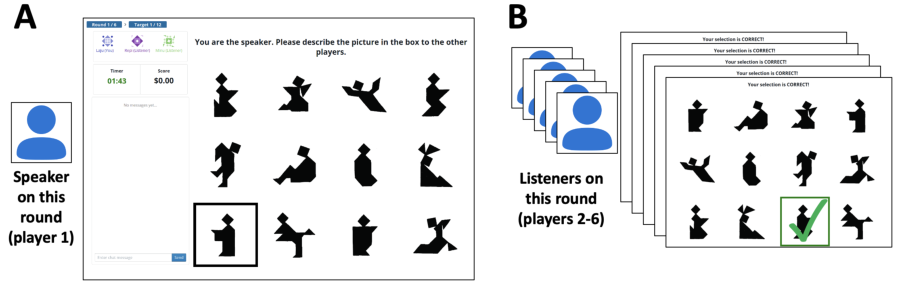
\includegraphics[width=1\linewidth]{figs/interface-1} 

}

\caption{All participants saw all 12 tangram images. (A) Speaker's view during selection phase. (B) During the feedback stage, speakers saw what figure each person chose, but listeners only learned if their selection was correct or incorrect. Listeners were not shown what other listeners chose. \label{game}}\label{fig:interface}
\end{figure*}

In this context, one approach for speakers is to `aim low' and produce utterances tailored to the least knowledgeable listener (\protect\hyperlink{ref-yoonAimLowMechanisms2018a}{\textbf{yoonAimLowMechanisms2018a?}}). For instance, in Yoon \& Brown-Schmidt (\protect\hyperlink{ref-yoonAdjustingConceptualPacts2014}{2014}), speakers developed conventions with one listener but then used longer descriptions with a new listener. Another strategy for speakers is to integrate across listeners and balance efficiency with informativeness by `aiming in the middle'. In Yoon \& Brown‐Schmidt (\protect\hyperlink{ref-yoonAudienceDesignMultiparty2019}{2019}), speakers communicating to a mixed group of 3 experienced listeners and 1 naive listener used shorter utterances and made fewer accommodations than they did in groups with a greater fraction of naive listeners. Both of these strategies predict that larger groups will be slower to converge than smaller groups.

Disagreements about how to conceptualize referents can also slow groups down. In (\protect\hyperlink{ref-weberCulturalConflictMerger2003}{\textbf{weberCulturalConflictMerger2003?}}), pairs of participants played a reference game with the same image sets before a listener switched groups and joined a different pair, making a group of three. The addition of the new listener slowed both listeners down for multiple rounds. When a listener switched groups, they brought preconceptions about how the pictures should be described which conflicted with how the speaker was used to describing the images. This result predicts that, with more perspectives in play, larger groups may have more difficulty agreeing on common conceptualizations.

In general, listeners expect speakers to maintain conventions and stick to descriptions that were similar to successful descriptions. However, listeners were not surprised to hear different descriptions of a familiar object if it came from a new speaker who had just entered the room (\protect\hyperlink{ref-metzingWhenConceptualPacts2003}{Metzing \& Brennan 2003}). It's unclear what this finding predicts about new speakers who are present as fellow listeners during prior blocks -- will listeners expect them to maintain conventions?

\hypertarget{experiment-1}{%
\section{Experiment 1}\label{experiment-1}}

For a first experiment, we extend the dyadic repeated reference game paradigm of Hawkins et al. (\protect\hyperlink{ref-hawkinsCharacterizingDynamicsLearning2020}{2020}) to games for 2--6 players who rotate between speaker and listener roles. This paradigm allowed us to test how the findings from dyadic interated reference games extend to larger groups and were influenced by group size. Additionally, to more closely examine how conventionalized names develop within groups and differ between groups, we used sentence embeddings to quantify the similarities of descriptions within and between groups over time.

\hypertarget{methods}{%
\subsection{Methods}\label{methods}}

Building on the methods of Hawkins et al. (\protect\hyperlink{ref-hawkinsCharacterizingDynamicsLearning2020}{2020}), we used Empirica (\protect\hyperlink{ref-almaatouqEmpiricaVirtualLab2020}{Almaatouq et al. 2020}) to create real-time multi-player reference games. In each game, one of the players started as the speaker who saw an array of tangrams with one highlighted (Figure \ref{game}A) and communicated which figure to click to the other players (listeners). After the speaker had identified each of the 12 images in turn, the speaker role rotated to another player and the process repeated with the same images. In total, there were 6 blocks, giving each player at least one chance to be the speaker. We recorded what participants said in the chat, as well as who selected what image and how long they took to make their selections.

\hypertarget{participants}{%
\subsubsection{Participants}\label{participants}}

We recruited participants between May and July 2021 using the Prolific platform; participants had all self-reported as fluent native English speakers on Prolific's demographic prescreen. Participants were paid \$7 for 2-player games, \$8.50 for 3-player games, \$10 for 4-player games, and \$11 for 5- and 6-player games (with the intention of a \$10 hourly rate), in addition to up to \$2.88 in performance bonuses. A total of 390 people each participated in one game.

\hypertarget{materials}{%
\subsubsection{Materials}\label{materials}}

We used the 12 tangram images used by Hawkins et al. (\protect\hyperlink{ref-hawkinsCharacterizingDynamicsLearning2020}{2020}) and Clark \& Wilkes-Gibbs (\protect\hyperlink{ref-clarkReferringCollaborativeProcess1986}{1986}) (see Figure \ref{game}). These images were displayed in a grid with order randomized for each participant (thus descriptions such as ``top left'' were ineffective as the image might be in a different place on the speaker's and listeners' screens). The same images were used every block.

\hypertarget{procedure}{%
\subsubsection{Procedure}\label{procedure}}

\begin{table}

\caption{\label{tab:overview}Summary of differences in experiments. Game size refers to the number of players per game. Speaker refers to whether there was one speaker the whole game or whether the speaker role rotated every block. Feedback is whether listeners saw only whether they were right or wrong or whether the additionally saw what other listeners had selected and what the correct answer was. Listener chat refers to whethers listeners could type freely in the chat or only communicate by pressing buttons to send four emojis to the chat. Continue games refers to whether games could continue (or start) with fewer than the requisite number of players; this was not intended to be a consequential manipulation, but was done to prevent games from ending if one player dropped out (an issue that was causing data loss in 6 player games). }
\centering
\begin{tabular}[t]{l|l|l|l|l|l}
\hline
Experiment & Game size & Speaker & Feedback & Listener chat & Continue games\\
\hline
1 & 2,3,4,5,6 & rotating & self only & text & no\\
\hline
2a & 6 & one speaker & self only & text & no\\
\hline
2b & 6 & rotating & self, others, \& correct & text & no\\
\hline
2c & 6 & rotating & self only & four emojis & no\\
\hline
3 thin & 2,6 & rotating & self only & four emojis & yes\\
\hline
3 thick & 2,6 & one speaker & self, others, \& correct & text & yes\\
\hline
\end{tabular}
\end{table}
\begin{table}

\caption{\label{tab:participants}The number of games in each experiment and condition. Complete games finished all 6 blocks; partial games ended early due to disconnections, but contributed at least one complete block of data. 6* indicates that some games started with fewer than 6 players or continued with fewer than 6 players after participants disconnected.}
\centering
\begin{tabular}[t]{l|l|r|r}
\hline
Experiment & Players & Complete & Partial\\
\hline
1 & 2 & 15 & 4\\
\hline
1 & 3 & 18 & 2\\
\hline
1 & 4 & 19 & 2\\
\hline
1 & 5 & 17 & 3\\
\hline
1 & 6 & 12 & 6\\
\hline
2a & 6 & 15 & 3\\
\hline
2b & 6 & 13 & 4\\
\hline
2c & 6 & 10 & 6\\
\hline
3: thin & 2 & 35 & 3\\
\hline
3: thin & 6* & 44 & 0\\
\hline
3: thick & 2 & 39 & 3\\
\hline
3: thick & 6* & 38 & 2\\
\hline
\end{tabular}
\end{table}

We implemented the experiment using Empirica, a Javascript-based platform for running real-time interactive experiments online (\protect\hyperlink{ref-almaatouqEmpiricaVirtualLab2020}{Almaatouq et al. 2020}). From Prolific, participants were directed to our website where they navigated through a self-paced series of instruction pages explaining the game. Participants had to pass a quiz to be able to play the game. They were then directed to a ``waiting room'' screen until their partners were ready.

Once the game started, participants saw screens like Figure \ref{game}A. Each trial, the speaker described the highlighted tangram image so that the listeners could identify and click it. All participants were free to use the chat box to communicate, but listeners could only click once the speaker had sent a message. Once a listener clicked, they could not change their selection. There was no signal to the speaker or other listeners about who had already made a selection.

Once all listeners had selected (or a 3-minute timer ran out), participants were given feedback (Figure \ref{game}B). Listeners learned whether they individually had chosen correctly or not; listeners who were incorrect were not told the correct answer. The speaker saw which tangram each listener had selected, but listeners did not. This feedback regime is different from Hawkins et al. (\protect\hyperlink{ref-hawkinsCharacterizingDynamicsLearning2020}{2020}) where listeners were shown what the right answer was during feedback. We made this change to prevent listeners from learning conventions purely as a memorized mapping between utterance and correct answer.

Listeners got 4 points for each correct answer; the speaker got points equal to the average of the listeners' points. These points translated into performance bonus at the end of the experiment.

In each block, each of the 12 tangrams was indicated to the speaker once. The same person was the speaker for an entire block, but participants rotated roles between blocks. Thus, over the course of the 6 blocks, participants were speakers 3 times in 2-player games, twice in 3-player games, once or twice in 4 and 5-player games, and once in 6-player games. Rotating the speaker was chosen to keep participants more equally engaged (the speaker role is more work), and to give a more robust test for reduction and convention.

After the game finished, participants were given a survey asking for optional demographic information and feedback on their experience with the game.

\hypertarget{data-pre-processing-and-exclusions}{%
\subsubsection{Data pre-processing and exclusions}\label{data-pre-processing-and-exclusions}}

Participants could use the chat box freely, which meant that the chat transcript contained some non-referential language. The first author skimmed through the chat transcripts, tagging utterances that did not refer to the current tangram. These were primarily pleasantries (``Hello''), meta-commentary about how well or fast the task was going, and confirmations or denials (``ok'', ``got it'', ``yes'', ``no''). We exclude these utterances from our analyses. Note that chat lines sometimes included non-referential words in addition to words referring to the tangrams (``ok, so it looks like a zombie'', ``yes, the one with legs''); these lines were retained intact.

Our intended sample size was 20 complete games in each group size, but we ended up with fewer due to games not filling or participants disconnecting early (Table \ref{parts}). We excluded incomplete blocks from analyses, but included complete blocks from partial games.

\hypertarget{modelling-strategy}{%
\subsubsection{Modelling strategy}\label{modelling-strategy}}

All models were run in brms CITE with weakly regularizing priors DESCRIBE

\hypertarget{results}{%
\subsection{Results}\label{results}}

\hypertarget{accuracy-and-speed}{%
\subsubsection{Accuracy and speed}\label{accuracy-and-speed}}

Our first question was whether accuracy and speed increased across groups of different sizes.

Most individuals were accurate in their selections, with accuracy rising across blocks (Figure \ref{accuracy}). In a logistic model of accuracy (correct.num\(\sim\) block \(\times\) numPlayers), participants are more accurate in later blocks (block: Est=0.38, CrI={[}0.25, 0.5{]}), and there was no strong effect of group size on accuracy (numPlayers: Est=-0.02, CrI={[}-0.08, 0.03{]}) or interaction between block and group size (block:numPlayers: Est=-0.01, CrI={[}-0.04, 0.01{]}).

Participants selected images faster in later blocks although there was wide variability. In a linear model of selection time (time\(\sim\) block \(\times\) numPlayers), participants got faster across blocks (block: Est=-10.03, CrI={[}-11.03, -9.03{]}) and were slightly slower in larger games (numPlayers: Est=1.03, CrI={[}0.4, 1.66{]}). This speed up is consistent with prior work by (\protect\hyperlink{ref-weberCulturalConflictMerger2003}{\textbf{weberCulturalConflictMerger2003?}}) which used speed as the dependent measure. Wide variability in selection time meant that especially for larger groups, there was a wide spread in how long it took groups to complete the experiment.

\begin{figure*}[t!]

{\centering \includegraphics[width=1\linewidth]{figs/triptych-acc-1} 

}

\caption{TODO}\label{fig:triptych-acc}
\end{figure*}

\hypertarget{reduction}{%
\subsubsection{Reduction}\label{reduction}}

\begin{figure*}[t!]

{\centering \includegraphics[width=1\linewidth]{figs/triptych-red-1} 

}

\caption{TODO}\label{fig:triptych-red}
\end{figure*}

The key phenomonenon of iterated reference games is that the descriptions to the target images shorten over the course of repetition. This pattern holds for the small groups in this experiment as well. The number of words produced by speakers decreases over the course of rounds, both in aggregate and for many individual groups (Figure \ref(fig:triptych-red)). Nonetheless, in some groups, a later speaker may be more verbose than an earlier speaker. Speakers make longer utterances in early blocks that reduce to shorter utterances in later blocks. From a linear model (words\(\sim\) block \(\times\) numPlayers~+ (block\textbar tangram)~+ (1\textbar playerId)~+ (1\textbar tangram\_group)~+ (block\textbar gameId)), the effect of being one block later is -3.35 (CrI={[}-4.58, -2.13{]}) words.

The overall effect of having more players in a group is 1.67 (CrI={[}0.68, 2.71{]}) words from the speaker per trial per additional player. There is no clear interaction between block and group size (block:numPlayers: Est=-0.1, CrI={[}-0.39, 0.18{]}). Larger groups saying more is consistent with predictions from audience design that with more listeners to accommodate, the speaker may use multiple conceptualizations, either initially as a hedge or in response to listener clarifications.

One potential concern is that group size correlates with whether the speaker has had the speaker role before (smaller groups repeat speakers more). To address this confound, we coded for whether the speaker has been speaker in an earlier block\footnote{words\(\sim\) block \(\times\) numPlayers~+ block \(\times\) speaker.repeat~+ (block\textbar tangram)~+ (1\textbar playerId)~+ (1\textbar tangram\_group)~+ (block\textbar gameId)}. Repeat speakers do use fewer words (speaker.repeat: Est=-8.55, CrI={[}-10.41, -6.79{]}), but there are still effects of group size (numPlayers: Est=1.63, CrI={[}0.58, 2.66{]}) and block (block: Est=-5.26, CrI={[}-6.84, -3.69{]}). The effects of block and repeat speaker are subadditive (block:speaker.repeat: Est=3.2, CrI={[}2.65, 3.78{]}), and there is minimal interaction between block and group size (block:numPlayers: Est=0.08, CrI={[}-0.22, 0.41{]}).

In our games (which had limited feedback), listeners who got a tangram wrong didn't have a way of knowing what the right answer was unless they asked for clarification in the chat. If a speaker got a tangram wrong as a listener in the previous block, they may not have known the conventional description that went with it, and thus were unlikely to follow the convention. If we assume that reduction is a sign of convention development, then speakers should say more words when they got the tangram wrong the previous block. We added prior errors as an additional predictor to our regression predicting number of words and found that speakers said more words for tangrams after they were incorrect (numPlayers: Est=2.18, CrI={[}0.93, 3.44{]}).

\hypertarget{role-of-listeners}{%
\subsubsection{Role of listeners}\label{role-of-listeners}}

Listeners often don't talk much, but are more likely to ask questions or make clarification in early blocks. In a linear regression for the number of words each listener said ( words\(\sim\) block \(\times\) numPlayers~+ (block\textbar tangram)~+ (1\textbar playerId)~+ (1\textbar tangram\_group)~+ (block\textbar gameId)), there was an effect of block (block: Est=-0.48, CrI={[}-0.79, -0.18{]}), but no clear effect of game size (numPlayers: Est=0.2, CrI={[}-0.13, 0.51{]}).

TODO say more about what sorts of utterances listeners make and stuff!!!!

\hypertarget{divergence}{%
\subsubsection{Divergence}\label{divergence}}

\begin{figure*}[t!]

{\centering \includegraphics[width=1\linewidth]{figs/triptych-div-1} 

}

\caption{TODO}\label{fig:triptych-div}
\end{figure*}

\hypertarget{examples-of-names}{%
\subsubsection{Examples of names}\label{examples-of-names}}

While most groups did form conventions for most tangrams, it's illustrative to look at a case where a group did not. Table \ref{diamond} shows the transcript of a 4-person group for a specific figure where they described it geometrically every round, leading to long and not very informative descriptions. Nearly all the figures have diamond heads, so this isn't a distinguishing feature, yet it is described. This illustrates the variability between groups, but also why conventions might be useful.

\begin{table}[H]

\caption{\label{tab:diamond}Excerpt from a group that did not reduce very much. The speaker for each round is marked with (S). Figure under discussion is row 3, column 3 in Figure \ref{game}A.\label{diamond}}
\centering
\begin{tabular}[t]{ll>{\raggedright\arraybackslash}p{16em}}
\toprule
Block & Person & Text\\
\midrule
1 & A(S) & Diamond on top. Body with no real arms or legs. The body is shaped like a boot with the diamond on top.\\
 & C & Is the boot pointed left or right?\\
2 & B(S) & diamond on top, large body beneath it. Left is a straight line all the way down, small variations on the right to the main body\\
3 & C(S) & Diamond in center on top. Left side straight, right side carved out like a vase.\\
4 & D(S) & Diamond head, flat topped body, straight on the left side with two triangles pointing out on the left\\
 & D(S) & *on the right\\
5 & A(S) & Diamond on top. Left side is straight, right side is obstructed, looks like a boot\\
 & B & what do you mean by obstructed?\\
 & A(S) & The left side of the body is right, right side has bents in it\\
6 & B(S) & Diamond on top of a long large body/rectangle. Left side is complete, right side has bits missing\\
\bottomrule
\end{tabular}
\end{table}

A different 4-person group had a member who during the first block shared the idea that the task would be easier if they explicitly gave ``codenames'' to the figures. The transcript for this group and one of the tangrams is shown in Table \ref{zigzag}. Of note, multiple speakers forget the assigned codename, demonstrating that meta-knowledge doesn't always help. This group also describes the figure in relation to another already-named figured. Nonetheless, the group successfully conventionalizes on a couple reduced names for this figure: ``zigzag'' and ``beggar''. This dual-naming of figures from multiple conceptual angles contributed by different speakers also occurs in other games.

\hypertarget{convergence}{%
\subsubsection{Convergence}\label{convergence}}

\begin{figure*}[t!]

{\centering \includegraphics[width=1\linewidth]{figs/triptych-conv-1} 

}

\caption{TODO}\label{fig:triptych-conv}
\end{figure*}

\hypertarget{interim-discussion}{%
\subsection{Interim Discussion}\label{interim-discussion}}

Experiment 1 sought to extend iterated reference games to groups of up to 6 players and look at how group size variation influenced different aspects of the reduction phenomena. Across group sizes, accuracy was high and increasing and descriptions reduced over the course of the game.

TODO comment on role of listeners and qualia

By using NLP tools, we took a quantified look at how partner-specific convergence of referring expressions happens.

TODO FIX ME

However, one limitation we observed was that the rotation of the speaker role causes speaker experience later in the game to confound with game size.

\hypertarget{experiment-2}{%
\section{Experiment 2}\label{experiment-2}}

After experiment 1, there were concerns about whether the results were dependent on any of the methods details. We were also interested in whether there were changes in knowledge or group communication that could support (or diminish) success, especially in the larger groups. To explore this, we ran 3 variants of the paradigm in experiment 1, varying different parameters. These were all run on small sets of 6 player groups.

TODO examples of prior literature that rotated or didn't rotate !!!
Previous literature varied on whether one person had the speaker role the entire game, or whether the two participants alternated speaker and listener roles in some way. For experiment 1, we went with rotating the speaker every block: we thought this would be percieved as more fair by participants, and we thought it would be a more stringent test of convergence to convention. However, in smaller groups, the speaker role would rotate back around, meaning that the speaker in later blocks would be more experienced in small games than in large games where speakers were usually first time speakers. We cannot disentangle the effects of group size from the effects of speaker experience. To address whether continuity in speakers might contribute to better performance, in experiment 2a we ran 6 player games with one person assigned to be the speaker the entire game.

Another point of variation in the literature is what sort of feedback is given. In particular, there is variation in whether participants were told what the right answer was when they were wrong (like in Hawkins et al. (\protect\hyperlink{ref-hawkinsCharacterizingDynamicsLearning2020}{2020})). In experiment 1, we opted for the minimum feedback, to make sure that participants had to negotiate and understand conventions, and could not just pick them up from the end of trial feedback. To see whether this mattered, in experiment 2b, we increased the amount of feedback, showing each participant what everyone had selected and what the right answer was.

Listener feedback to the speaker in the form of some backchannel, is implicated in the theoretical literature as being important to convention formation TODO CITES. We were interested in whether limiting this backchannel would be a way to push around the reduction pattern and significantly change it. We were worried that entirely removing the backchannel would make the game too unfun and encourage random clicking or quitting of the speaker was just talking into the void. As a compromise between limiting the backchannel and maintaining playability, we switched to giving the listeners a discrete backchannel consisting of 4 emojis, expressing whether they understood, whether they wanted more details, whether they were totally confused, or whether they were amused (TODO figure with emojis and their meanings). These options were based on the common valences expressed in the free chat of listeners from experiment 1. Thus, in 2c, listeners could not contribute questions or content to the discourse, but the speaker still had some feedback on whether the listeners were understanding.

\hypertarget{methods-1}{%
\subsection{Methods}\label{methods-1}}

\hypertarget{participants-1}{%
\subsubsection{Participants}\label{participants-1}}

All participants were self-reported fluent native English speakers who had not participated in experiment 1.
All experiment 2 games were 6-player games. All games had a base pay of \$11, in addition to up to \$2.88 in performance bonuses for each player.
Experiment 2a was run in March and April 2022, and the speaker got an additional \$2 bonus to compensate for the increased effort of being the only speaker.
Experiment 2b was run in July 2022 and Experiment 2c was run in August 2022.

A total of N people participated in experiment 2.

\hypertarget{materials-1}{%
\subsubsection{Materials}\label{materials-1}}

The materials were the same as in experiment 1.

\hypertarget{procedure-1}{%
\subsubsection{Procedure}\label{procedure-1}}

Experiment 2 consisted of three different variations on Experiment 1, so we describe the differences from the Experiment 1 procedure. For the differences between games see TABLE TODO.

The only change for experiment 2a was that one person was designated the speaker for the entire game.

For experiment 2b, feedback was changed so that all participants in the feedback stage saw the speaker view showing who selected what and what the right answer was. Listeners still saw text saying whether they individually were correct or wrong.

For experiment 2c, we altered the chatbox interface for listeners. Instead of a textbox, listeners had 4 buttons, each of which sent a different emoji to the chat. Listeners were given suggested meanings for the 4 emojis during instructions. They could send the emojis as often as desired, for instance, initially indicating confusion, and later indicating understanding. In addition, we added notifications that appeared in the chat box saying when a player had made a selection.

\hypertarget{results-1}{%
\subsection{Results}\label{results-1}}

\hypertarget{accuracy}{%
\subsubsection{Accuracy}\label{accuracy}}

\hypertarget{reduction-1}{%
\subsubsection{Reduction}\label{reduction-1}}

\hypertarget{divergence-1}{%
\subsubsection{Divergence}\label{divergence-1}}

\hypertarget{convergence-1}{%
\subsubsection{Convergence}\label{convergence-1}}

\hypertarget{emoji-usage}{%
\subsubsection{Emoji usage ?}\label{emoji-usage}}

\hypertarget{interim-discussion-1}{%
\subsection{Interim discussion}\label{interim-discussion-1}}

\hypertarget{experiment-3}{%
\section{Experiment 3}\label{experiment-3}}

Based on the results of experiment 2, it seemed that speaker continuity helped groups, and that more feedback maybe helped groups, while limiting the backchannel reduced accuracy and reduction. These results are tentative as we had a limited number of groups in each of these conditions. To more robustly demonstrate that the reduction phenomena were sensitive to these variations in group structure and coherency and to investigate how they interacted with group size, we conducted a better powered experiment. As these experiments are expensive to run, we did not do a full-factorial design; instead, we collapsed the three sources of variation into a ``thick-channel'' condition, combining single speaker, high feedback, and text backchannel, the settings that give richer feedback and knowledge, and a ``thin-channel'' condition, which was the opposite (same condition as 2c above). We crossed these two conditions with group size: either 2 or 6 player groups, picking the extreme values from experiment 1.

We aimed for 40 games in each of these 4 cells. We had previously experienced problems with attrition in 6-player games, as when one or more participants quit, the game discontinued on everyone, leading to fewer games with data from the entire game. To mitigate this, we reprogrammed the game to instead try to keep the game going with the participants who were left (and to start games even if they hadn't filled completely).

\hypertarget{methods-2}{%
\subsection{Methods}\label{methods-2}}

\hypertarget{participants-2}{%
\subsubsection{Participants}\label{participants-2}}

All participants were self-reported fluent native English speakers who had not participated in experiment 1 or experiment 2.

Experiment 3 was run in October 2022. Participants in 2-player games were paid \$7 base pay, and participants in 6-player games were paid \$11 base pay. Speakers in the 6-player thick condition were given a \$2 bonus, and all participants could early up to \$2.88 in performance bonus. A total of M people participated.

\hypertarget{materials-2}{%
\subsubsection{Materials}\label{materials-2}}

The materials were the same as in experiment 1.

\hypertarget{procedure-2}{%
\subsubsection{Procedure}\label{procedure-2}}

The thin channel condition was the same as with experiment 2c, described above.

The thick channel condition was the same as experiment 1, except that one person was designated the speaker throughout, and all participants saw the speaker view for feedback.

TODO confirm. Across both conditions, messages were sent to the chat to indicate when a participant had made a selection.

The large change was behind the scenes, to handle games continuing after a participant had quit. Participants were identified as disconnected if their computer was not responding to the server for YY seconds (for instance if they closed the tab and did not reopen it quickly). If the person who disconnected was a listener, they were just removed, and they were skipped over by the speaker rotation (if applicable). If the person who disconnected was a speaker, that trial was discontinued as there was no way for listeners to get more information, and another person was assigned as speaker for the remainder of the block (or remainder of the game, depending on condition).

TODO figure out how this interacts with the full blocks thing!!! Maybe we should break the pre-reg? (in general?, only here?)

TODO the actual distribution of game sizes!!

TODO add pre-registrations everywhere

Note: when skimming transcripts to tag non-referential utterances, we noticed that one game in the 6-player thick game had a speaker who did not give any sort of coherent descriptions, even with substantial listener prompting. We excluded this game from analyses.

\hypertarget{results-2}{%
\subsection{Results}\label{results-2}}

TODO there's a note saying to rerun these models for longer with more extensive mixed effects!! (at least of reduction model)

\hypertarget{accuracy-model}{%
\subsection{Accuracy model}\label{accuracy-model}}

\begin{verbatim}
## # A tibble: 8 x 4
##   Term                         Estimate `Credible Interval` `P-value equivalent`
##   <chr>                           <dbl> <chr>                              <dbl>
## 1 channelthin                     -0.34 [-0.66, -0.01]                     0.044
## 2 channelthin:gameSize6            0.22 [-0.16, 0.6]                       0.25 
## 3 gameSize6                       -0.44 [-0.73, -0.16]                     0.002
## 4 Intercept                        1.79 [1.45, 2.13]                       0    
## 5 repNum                           0.55 [0.42, 0.67]                       0    
## 6 repNum:channelthin              -0.09 [-0.26, 0.07]                      0.28 
## 7 repNum:channelthin:gameSize6    -0.02 [-0.23, 0.18]                      0.82 
## 8 repNum:gameSize6                -0.17 [-0.33, -0.02]                     0.022
\end{verbatim}

TODO

\hypertarget{reduction-of-words}{%
\subsubsection{Reduction of words}\label{reduction-of-words}}

This model was run with 2 player thick as the default. The effect of being one block later for 2 player thick games is -2.33 (CrI={[}-3.03, -1.64{]}). TODO

\hypertarget{sbert-models}{%
\subsection{Sbert models}\label{sbert-models}}

\hypertarget{divergence-2}{%
\paragraph{Divergence}\label{divergence-2}}

\begin{verbatim}
## # A tibble: 8 x 4
##   Term                         Estimate `Credible Interval` `P-value equivalent`
##   <chr>                           <dbl> <chr>                              <dbl>
## 1 channelthin                      0.01 [0.01, 0.02]                           0
## 2 channelthin:gameSize6           -0.03 [-0.04, -0.02]                         0
## 3 gameSize6                        0.05 [0.05, 0.05]                           0
## 4 Intercept                        0.41 [0.37, 0.45]                           0
## 5 repNum                          -0.02 [-0.02, -0.02]                         0
## 6 repNum:channelthin               0    [0, 0]                                 0
## 7 repNum:channelthin:gameSize6     0.02 [0.02, 0.02]                           0
## 8 repNum:gameSize6                -0.01 [-0.01, -0.01]                         0
\end{verbatim}

TODO

\hypertarget{convergence-2}{%
\section{Convergence}\label{convergence-2}}

\begin{verbatim}
## # A tibble: 16 x 4
##    Term                                                  Estim~1 Credi~2 P-val~3
##    <chr>                                                   <dbl> <chr>     <dbl>
##  1 channelthin                                             -0.01 [-0.19~    0.93
##  2 channelthin:gameSize6                                    0.04 [-0.14~    0.66
##  3 channelthin:gameSize6:samespeakersame_speaker            0.02 [-0.17~    0.86
##  4 channelthin:samespeakersame_speaker                      0.01 [-0.19~    0.93
##  5 earlier                                                  0.06 [-0.11~    0.51
##  6 earlier:channelthin                                     -0.01 [-0.19~    0.92
##  7 earlier:channelthin:gameSize6                           -0.02 [-0.19~    0.87
##  8 earlier:channelthin:gameSize6:samespeakersame_speaker    0    [-0.19~    0.96
##  9 earlier:channelthin:samespeakersame_speaker             -0.01 [-0.19~    0.91
## 10 earlier:gameSize6                                       -0.01 [-0.19~    0.96
## 11 earlier:gameSize6:samespeakersame_speaker                0.01 [-0.16~    0.88
## 12 earlier:samespeakersame_speaker                          0.02 [-0.17~    0.87
## 13 gameSize6                                               -0.06 [-0.24~    0.53
## 14 gameSize6:samespeakersame_speaker                       -0.01 [-0.2,~    0.88
## 15 Intercept                                                0.53 [0.34,~    0   
## 16 samespeakersame_speaker                                  0.06 [-0.13~    0.54
## # ... with abbreviated variable names 1: Estimate, 2: `Credible Interval`,
## #   3: `P-value equivalent`
\end{verbatim}

\hypertarget{emoji-usage-1}{%
\subsubsection{Emoji usage}\label{emoji-usage-1}}

\hypertarget{general-discussion}{%
\section{General Discussion}\label{general-discussion}}

this isn't the only group dynamic; could imagine situations where listeners can see each others work collaborate (point to each other what htey think, perhaps see feedback from speaker to one listener) which might make things reduce much faster

The emergence of conventions has been a key case study for communication more broadly. Yet this issue has -- for the most part -- been studied only in dyadic communication. While some studies have examined aspects of convention formation in larger groups (e.g., \protect\hyperlink{ref-yoonAdjustingConceptualPacts2014}{Yoon \& Brown-Schmidt 2014}, \protect\hyperlink{ref-yoonAudienceDesignMultiparty2019}{Yoon \& Brown‐Schmidt 2019}), basic descriptive work has not yet investigated how group size changes the dynamics of interaction in a standard referential communication task, in part because such tasks can be difficult to administer to larger groups. Taking advantage of a new online multi-player experiment platform, we ran repeated reference games with groups of 2--6 players and characterized the nature of group performance.

Consistent with dyadic games, listeners' selection accuracy increased over blocks at the same time as listeners sped up their selections (question 1).
Crucially, speakers reduced the length of their descriptive utterances as they conventionalized on concepts for each image (question 2). Because speakers rotated, this reduction finding is robust: not only did speakers say less in later repetitions than they themselves said earlier, speakers later in the order said less than speakers earlier in the rotation. This reduction varied with group size; smaller groups used shorter utterances, but group size did not significantly interact with block (question 3). The trajectory of reduction also depended on whether the current speaker correctly identified the tangram in the prior block and whether the current speaker was new to being speaker. This pattern is consistent with both the `aim low' and `aim middle' hypotheses from previous work (\protect\hyperlink{ref-yoonAdjustingConceptualPacts2014}{Yoon \& Brown-Schmidt 2014}, \protect\hyperlink{ref-yoonAudienceDesignMultiparty2019}{Yoon \& Brown‐Schmidt 2019}).

What was specifically different across group sizes? Smaller groups showed more agreement in how each tangram was identified across blocks (question 4), coming to consensus earlier: Their overlap between descriptions in the first 5 blocks to the final block was higher, and words in the final block tended to originate earlier. The greater diversity in how tangrams were described in larger groups could be explained by slower convergence to a convention or parallel competing conceptualizations favored by different speakers. Larger groups have more people for the speaker to communicate to, but also more people who might interrupt with questions, and more people who have opinions about what each image looks like. Bigger groups differ from smaller groups in a number of ways, however, and disentangling these differences is an area for future work.

Group interactions are rich, and this experiment is necessarily a schematic simplification with a number of limitations. Real-life situations vary widely in who the interlocuters are, their relationships, their goals, and their environment (\protect\hyperlink{ref-carletta1998}{Carletta et al. 1998}, \protect\hyperlink{ref-fay2000}{Fay et al. 2000}). Our participants were a convenience sample of Prolific workers who were strangers to each other; thus we miss richness that could come from prior relationships or shared community. Reference is only one goal out of many possible communicative goals, and the tangram images are artificial.
We provided less feedback than previous studies such as Hawkins et al. (\protect\hyperlink{ref-hawkinsCharacterizingDynamicsLearning2020}{2020}); this regime imitates situations where interlocutors can't show each other examples, but it's not representative of all communicative environments. Further, our text-based online paradigm meant that participants' individual identities were not especially salient. In sum, communication takes place in a plethora of situations; our experiment provides some insights, but also misses many complexities that should be a focus of further experiments.

The experimental paradigm presented here could be a valuable tool to disentangle the mechanisms of group size and determine which design parameters are relevant to reduction. Luckily, with an online implementation, recruiting for and running experiments is feasible, and thus it will be possible to iterate on this experiment to determine how far the patterns generalize. While much is left to be explored, this initial data set provides a rich corpus of how humans adapt language dynamically to communicate.

\hypertarget{limitations}{%
\subsection{Limitations}\label{limitations}}

\hypertarget{references}{%
\section{References}\label{references}}

\setlength{\parindent}{-0.1in} 
\setlength{\leftskip}{0.125in}

\noindent

\hypertarget{refs}{}
\begin{CSLReferences}{1}{0}
\leavevmode\vadjust pre{\hypertarget{ref-almaatouqEmpiricaVirtualLab2020}{}}%
Almaatouq A, Becker J, Houghton JP, Paton N, Watts DJ, Whiting ME (2020) \href{http://arxiv.org/abs/2006.11398}{Empirica: A virtual lab for high-throughput macro-level experiments}. \emph{ArXiv200611398 Cs}

\leavevmode\vadjust pre{\hypertarget{ref-carletta1998}{}}%
Carletta J, Garrod S, Fraser-Krauss H (1998) Placement of {Authority} and {Communication Patterns} in {Workplace Groups}: {The Consequences} for {Innovation}. \emph{Small Group Research} \textbf{29}:531--559. doi:\href{https://doi.org/10.1177/1046496498295001}{10.1177/1046496498295001}

\leavevmode\vadjust pre{\hypertarget{ref-clarkReferringCollaborativeProcess1986}{}}%
Clark HH, Wilkes-Gibbs D (1986) \href{http://www.speech.kth.se/~edlund/bielefeld/references/clark-and-wilkes-gibbs-1986.pdf}{Referring as a collaborative process}. \emph{Cognition}

\leavevmode\vadjust pre{\hypertarget{ref-fay2000}{}}%
Fay N, Garrod S, Carletta J (2000) Group {Discussion} as {Interactive Dialogue} or as {Serial Monologue}: {The Influence} of {Group Size}. \emph{Psychol Sci} \textbf{11}:481--486. doi:\href{https://doi.org/10.1111/1467-9280.00292}{10.1111/1467-9280.00292}

\leavevmode\vadjust pre{\hypertarget{ref-haber2019}{}}%
Haber J, Baumgärtner T, Takmaz E, Gelderloos L, Bruni E, Fernández R (2019) The {PhotoBook Dataset}: {Building Common Ground} through {Visually-Grounded Dialogue}. In: \emph{Proc. 57th {Annu}. {Meet}. {Assoc}. {Comput}. {Linguist}.} {Association for Computational Linguistics}, {Florence, Italy}, p 1895--1910. Available from: \url{https://www.aclweb.org/anthology/P19-1184} {[}Last accessed 1 February 2022{]}. doi:\href{https://doi.org/10.18653/v1/P19-1184}{10.18653/v1/P19-1184}

\leavevmode\vadjust pre{\hypertarget{ref-hawkinsCharacterizingDynamicsLearning2020}{}}%
Hawkins RD, Frank MC, Goodman ND (2020) \href{http://arxiv.org/abs/1912.07199}{Characterizing the dynamics of learning in repeated reference games}. \emph{ArXiv191207199 Cs}

\leavevmode\vadjust pre{\hypertarget{ref-kraussChangesReferencePhrases1964}{}}%
Krauss RM, Weinheimer S (1964) Changes in reference phrases as a function of frequency of usage in social interaction: A preliminary study. \emph{Psychon Sci} \textbf{1}:113--114. doi:\href{https://doi.org/10.3758/BF03342817}{10.3758/BF03342817}

\leavevmode\vadjust pre{\hypertarget{ref-metzingWhenConceptualPacts2003}{}}%
Metzing C, Brennan SE (2003) When conceptual pacts are broken: {Partner-specific} effects on the comprehension of referring expressions. \emph{Journal of Memory and Language} \textbf{49}:201--213. doi:\href{https://doi.org/10.1016/S0749-596X(03)00028-7}{10.1016/S0749-596X(03)00028-7}

\leavevmode\vadjust pre{\hypertarget{ref-schober1989}{}}%
Schober MF, Clark HH (1989) Understanding by addressees and overhearers. \emph{Cognitive Psychology} \textbf{21}:211--232. doi:\href{https://doi.org/10.1016/0010-0285(89)90008-X}{10.1016/0010-0285(89)90008-X}

\leavevmode\vadjust pre{\hypertarget{ref-tolins2016}{}}%
Tolins J, Fox Tree JE (2016) Overhearers {Use Addressee Backchannels} in {Dialog Comprehension}. \emph{Cogn Sci} \textbf{40}:1412--1434. doi:\href{https://doi.org/10.1111/cogs.12278}{10.1111/cogs.12278}

\leavevmode\vadjust pre{\hypertarget{ref-traum2004}{}}%
Traum D (2004) Issues in {Multiparty Dialogues}. In: Dignum F (ed) \emph{Advances in {Agent Communication}}. {Springer Berlin Heidelberg}, {Berlin, Heidelberg}, p 201--211. Available from: \url{http://link.springer.com/10.1007/978-3-540-24608-4_12} {[}Last accessed 1 February 2022{]}. doi:\href{https://doi.org/10.1007/978-3-540-24608-4_12}{10.1007/978-3-540-24608-4\_12}

\leavevmode\vadjust pre{\hypertarget{ref-yoonAdjustingConceptualPacts2014}{}}%
Yoon SO, Brown-Schmidt S (2014) Adjusting conceptual pacts in three-party conversation. \emph{Journal of Experimental Psychology: Learning, Memory, and Cognition} \textbf{40}:919--937. doi:\href{https://doi.org/10.1037/a0036161}{10.1037/a0036161}

\leavevmode\vadjust pre{\hypertarget{ref-yoonAudienceDesignMultiparty2019}{}}%
Yoon SO, Brown‐Schmidt S (2019) Audience {Design} in {Multiparty Conversation}. \emph{Cogn Sci} \textbf{43}:e12774. doi:\href{https://doi.org/10.1111/cogs.12774}{10.1111/cogs.12774}

\end{CSLReferences}


\end{document}
